%%%%%%%%%%%%%%%%%%%%%%%%%%%%%%%%%%%%%%%%%%%%%%%%%%%%%%%%%%%%%%%%%%%%%%%%
% TFG: Vigilancia Tecnológica y Minería de Opiniones en RRSS
% Escuela Técnica Superior de Ingenierías Informática y de Telecomunicación
% Realizado por: Miguel Keane Cañizares
% Contacto: miguekeca@correo.ugr.es 
%%%%%%%%%%%%%%%%%%%%%%%%%%%%%%%%%%%%%%%%%%%%%%%%%%%%%%%%%%%%%%%%%%%%%%%%

\chapter{Implementación}

La mayor parte del proceso de implementación estará enfocado a la creación de los scripts que sean necesarios. Primero implementaremos un programa al que llamaremos \textit{ladrón de tweets} el cual será el encargado de obtener la información de Twitter, crear una base de datos MongoDB y almacernar los datos obtenidos en la misma. 


\subsection{Ladrón de Tweets}

La función de este script será la conexión con la API de Twitter, la escucha de tweets y su correcto almacenamiento en una base de datos MongoDB. La librerías más destacables utilizadas son: 
\begin{itemize}
	\item Pymongo\cite{Pymongo}: Librería para gestionar las conexiones con la base de datos MongoDB
	\item Tweepy\cite{Tweepy}: Librería para gestionar la conexión con la API de Twitter
\end{itemize}



Es necesario crear y conectarse a la base de datos MongoDB, en la cuál almacenaremos toda la información que posteriormente será descargada. 

\begin{figure}[h]
	\centering
	\includegraphics[scale=1.5]{imagenes/crearMongodb-ladron.png}
	\caption{Inicialización de base de datos MongoDB}
	\label{fig:crear-mongodb}
\end{figure}


Posteriormente es necesario declarar las variables que emplearemos al usar la API de Twitter. El idioma seleccionado, las claves de acceso y las palabras claves que deseamos descargar. 



Llegado este punto,nos conectaremos con la API de Twitter mediante las funcionalidades de Tweepy, usando las variables previamente declaradas. Con la función Stream, lo que hacemos es ponerlo en modo escucha, es decir, accederemos a los tweets que sean escritos en el tiempo de ejecución y estos serán los que descarguemos. Debemos incluir el modo \textit{$tweet\_mode$=extended} el cual es necesario porque en caso contrario solo se descargarán los primeros 140 caracteres del tweet, añadiendo información incompleta y por lo tanto desechable en la base de datos. 

\begin{figure}[h]
	\centering
	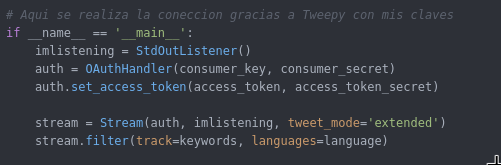
\includegraphics[scale=.5]{imagenes/inicio-sesion-ladron.png}
	\caption{Inicio de sesión en la API de Twitter}
	\label{fig:inicio-sesion-ladron}
\end{figure}


En la función \textit{StdOutListener()} tendremos la parte clave del script, en donde extraeremos la información del tweet y la almacenaremos en MongoDB. Evitaremos descargar los Retweets, ya que por experiencia, estos ensucian la base de datos, debido a que los retweets suponen una repetición de información, no aportando nada nuevo e invalidando en parte los resultados de su posterior análisis. 

















\subsection{Análisis de Sentimientos}


Una vez existe una base de datos MongoDB hay que enviarla a analizar a MeaningCloud haciendo uso de su API. Tras su análisis, obtendremos una información que será almacenada por partida doble, para facilitar la reutilización de la misma. Crearemos una colección diferente dentro de la base de datos MongoDB ya existente, a la que denominaremos \textit{concepts} y a la par se creará un archivo CSV en el cual almacenaremos toda la información para facilitar su posterior análisis. 


También será necesario indicar las claves de acceso para la API de MeaningCloud y la dirección url de acceso a la misma. 


\begin{figure}[H]
	\centering
	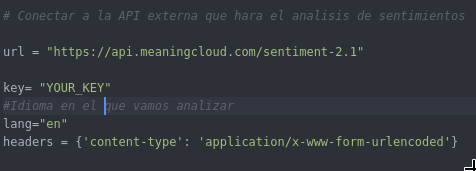
\includegraphics[scale=.35]{imagenes/key-analisis.png}
	\caption{Declaración de variables necesarias para la API de MeaningCloud}
	\label{fig:key-analisis}
\end{figure}




El código recorrerá toda la colección \textit{tweets} de la base de datos MongoDB, mandando únicamente el texto de los tweets a MeaningCloud, pues es la información que deberá ser analizada. Extraemos la información de utilidad de la respuesta y la almacenamos en diferentes variables. Dichas variables son:

\begin{itemize}
	\item \textbf{Confidence:} Es el valor de fiabilidad del análisis. MeaningCloud asigna un valor de 0-100, siendo 100 lo más fiable posible a la calidad de su análisis. Sólo cogeremos los resultados de los análisis aceptables, es decir, que tengan un valor superior a 90.
	\item \textbf{Score\_tag:} Posiblemente la variable más importante del análisis. Puesto que clasificará entre muy positivo y muy negativo el tono emocional del texto analizado. Su rango de polaridad es: 
	\begin{itemize}
		\item P+: Muy positivo
		\item P: Positivo
		\item NEU: Neutral
		\item N: Negativo
		\item N+: Muy negativo
		\item NONE: Ninguno, no se le ha detectado ningún tono emocional al texto.
	\end{itemize}
	\item \textbf{Agreement:} Si hay más de un sentimiento detectado en el texto, si estos sentimientos tienen el mismo tono emocional o no. 
	\item \textbf{Subjectivity:} Subjetividad. Indica si el texto es objetivo o subjetivo.
	\item \textbf{Irony:} Indica si el texto es irónico o no. La experiencia en este proyecto ha aconsejado ignorar esta variable por resultar su tasa de acierto muy baja o nula. 
	\item \textbf{Sentimented\_Entity\_List:} Lista de entidades en el texto que tienen una polaridad, es decir, generan un tono emocional en el autor. Nombres de compañías de servicio, ciudades, países, nombres de usuario. Reconoce un gran rango de entidades. 
	\item \textbf{Sentimented\_Concept\_List:} Lista de conceptos en el texto los cuales tienen polaridad concreta. 
\end{itemize}

De todos estos datos, solo serán almacenados \textit{Score\_tag}, \textit{Agreement}, \textit{Subjectivity} e \textit{Irony}.  Y solo se almacenarán si la confianza está por encima de un umbral de aceptabilidad. Estos datos serán guardados en un fichero CSV y en una nueva colección \textit{concepts} de MongoDB. 

También es interesante resaltar que el análisis de MeaningCloud\cite{MeaningCloud} no admite emojis y a veces simplemente devuelve que no ha podido analizar el texto introducido. Por lo que ha sido necesario gestionar excepciones para asegurarnos de que el programa no deja de ejecutarse.


NOTA: Existe otro script llamado \textbf{analisis-desde-nombre}, el cual es casi idéntico al anteriormente descrito cuya única diferencia es que podemos analizar la base de datos desde un usuario determinado. Por lo que si hay un error, como puede ser una perdida de conexión, será tan trivial como abrir el fichero CSV, buscar el nombre del último usuario añadido al fichero y escribir dicho nombre en la comprobación del script para continuar la búsqueda sin repetir tweets y sin perder información. 



\subsection{Nubes de palabras y representaciones gráficas}

Este script gestionará el estudio de los resultados del análisis de sentimientos de MeaningCloud. Creará gráficas y nubes de palabras donde se podrán ver que polaridades han sido las más frecuentes y que palabras han sido las más utilizadas. Para ello el script recorrerá cada fichero CSV con los resultados de MeaningCloud. Para este script, las librerías más relevantes que se han usado son: 


\begin{itemize}
	\item NumPy\cite{Numpy}: Extensión de python específica para darle mayor soporte para vectores y matrices. Constituye una librería de funciones matemáticas de alto nivel.
	\item Pandas\cite{Pandas}: Estrechamente relacionada con la bibliotea NumPy está orientada a la manipulación y análisis de datos. 	
	\item Matplotlib\cite{Hunter:2007}: biblioteca para la generación de gráficos a partir de datos contenidos en listas o arrays, relacionada también con la extensión NumPy. Diseñada para ser similar a la utilizada en MATLAB.
	\item PIL\cite{Pillow}: Python Imaging Lybrary, es una biblioteca que añade soporte para abrir, manipular y almacenar muchos formatos de imagen distintos. 
	
\end{itemize}


Al comienzo del código estarán las variables que habrá que modificar para seleccionar los ficheros adecuados. Hay que introducir el fichero CSV que será analizado, el nombre de la gráfica de barras que será generada, la imagen que se utilizará como modelo para la creación de la nube de palabras y el nombre que queremos darle a la nube de palabras que generaremos. 

\begin{figure}[H]
	\centering
	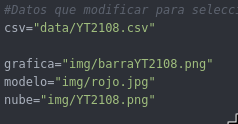
\includegraphics[scale=.5]{imagenes/datosWords.png}
	\caption{Datos que deberán editarse cada ejecución}
	\label{fig:datos-words}
\end{figure}

El código extraerá la información del fichero CSV deseado con la función \textit{read\_csv()} de la librería Pandas. Como información añadida mostrará por pantalla cuantos tweets hay de cada polaridad, desde muy positivo a muy negativo, también hará un recuento de las palabras que haya en la totalidad de los tweets. Los cuales se unificarán todos en una sola variable gracias a un bucle y a la facilidad de manipulación de datos que ofrece Pandas.

Haciendo uso de las funciones de Matplotlib\cite{Hunter:2007}, se generarán unas gráficas de barras. En estos resultados se omitirán los valores de polaridad "NONE". Pues estos son aquellos tweets que por la razón que sea no se les ha detectado ninguna polaridad, por lo tanto no proporcionan información relevante para el estudio de resultados. 
 
 Finalmente para este fragmento, se le introduce una imagen previamente seleccionada, la cual hará de plantilla para la posterior generación de la nube de palabras, es decir, en vez de usar la forma en la que aparece por defecto, empleará la forma y colores de dicha imagen. La imagen deberá estar en formato RPG, pues gracias a Numpy\cite{Numpy} se generará una máscara con ella transformada en un array de datos. La función array de Numpy convierte la imagen en un vector de datos comprendidos en un rango de 0-255 que contendrán la información de la misma en un formato que el algoritmo pueda procesar.




Una opción importante para la creación de la nube de palabras es la asignación de Stopwords, los cuales serán palabras que no se mostrarán en el fichero que se cree. Puesto que hay palabras que debido al formato de los tweets son propensas a aparecer mucho, podemos quitarlas para obtener un resultado más satisfactorio. Por ejemplo, en una base de datos acerca de Netflix, es asumible que todos los tweets contendrán la palabra Netflix, pues esa ha sido la palabra clave de búsqueda. Con esta información, lo apropiado será excluir la palabra Netflix de la nube de palabras, pues de no hacerlo el algoritmo la detectaría repetida múltiples veces y la mostraría en grande. 

\begin{figure}[H]
	\centering
	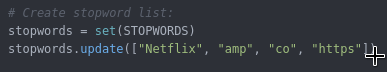
\includegraphics[scale=.7]{imagenes/stopword.png}
	\caption{Adición de Stopwords al WordCloud}
	\label{fig:stopwords}
\end{figure}


Por último, es preciso la generación del WordCloud en sí. Llamando a la función \textit{WordCloud()} en la que introducimos los parámetros deseados, entre los que destacan el número máximo de palabras que generaremos, la máscara que indicará la forma que debe tomar la nube, los stopwords que se han añadido con prioridad, el grosor de los bordes (de tenerlos) de la plantilla y el color de dichos bordes. Con la función \textit{ImageColorGenerator()} a la cual se le añade como parámetro la máscara generada con NumPy, indicará qué colores tomarán las palabras al pintar la figura. Para finalizar, con las funcionalidades de Matplotlib se pintará la imagen, habiendo de indicarle el tamaño de la figura resultante y pasarle la variable de wordcloud que contiene las palabras y por parámetro el color que deseamos que tengan dichas palabras para respetar el formato original. Finalmente, guarda la figura con el nombre y formato deseado y la muestra por pantalla. 











